\documentclass{article}

%%%%%%%%%%%%%%%%%%%%%%%%%%%%%%%%%%%%%%%%%%%%%%%%%%%%%%%%%%%%%%%%%
%package

%geometry
\usepackage[a4paper]{geometry}%调整页面边距
\geometry{left=3cm,right=3cm,top=3cm,bottom=3cm}
\linespread{1.5}
\usepackage{fancyhdr}%梦幻页眉

%fonts
\usepackage{fontspec}%字体库
\defaultfontfeatures{Mapping=tex-text}
\usepackage{xunicode,xltxtra}
\usepackage[BoldFont,SlantFont,CJKnumber,CJKchecksingle]{xeCJK}  % \CJKnumber{12345}: 一万二千三百四十五
\usepackage{CJKfntef}
\usepackage{bm} %公式中的粗体字符\boldsymbol
\usepackage{pifont}

%color
\usepackage{color,xcolor}
\definecolor{GREEN}{RGB}{25,180,68}
\definecolor{YELLOW}{RGB}{255,255,224}
\definecolor{BLUE}{RGB}{9,148,234}
\definecolor{RED}{RGB}{139,0,0}
\definecolor{DRED}{RGB}{128,0,0}
\definecolor{GREY}{RGB}{128,128,128}
\usepackage[pagecolor={YELLOW}]{pagecolor}%设置页面底色

%math
\usepackage{amsmath,amsfonts,amssymb}

%graphics
\usepackage[americaninductors,europeanresistors]{circuitikz}
\usepackage{tikz}%可以绘制各种坐标图,方格图
\usetikzlibrary{positioning,arrows,shadows,shapes,calc,mindmap,trees,backgrounds}  % placements=positioning
\usepackage{graphicx}%\includegraphics插图命令
\usepackage{subfigure}  %%图形或表格并排排列

% table
\usepackage{colortbl,dcolumn}  %% 彩色表格
\usepackage{multirow}
\usepackage{multicol}
\usepackage{booktabs}

% code
\usepackage{fancyvrb}%漂亮的代码包
\usepackage{listings}%加入代码

% ref
\usepackage{hyperref}%扩展参考文献,目录功能和加入超链接。

% title
\usepackage{titlesec}%花哨的章节标题

\usepackage{etoolbox}
\makeatletter
\patchcmd{\ttlh@hang}{\parindent\z@}{\parindent\z@\leavevmode}{}{}
\patchcmd{\ttlh@hang}{\noindent}{}{}{}
\makeatother%titlesec旧版本无编号问题


\titleformat
{\section} % command
[display] % shape
{\bfseries\Large} % format
{第\ \thesection 章\ } % label
{0.3ex} % sep
{
    \rule{\textwidth}{1pt}
    \vspace{1ex}
    \centering
} % before-code
[
\vspace{-2ex}%
\rule{\textwidth}{1pt}
] % after-code


%tightly-packed lists
\usepackage{mdwlist}
\usepackage{verbatim}%comment命令的注释包
\usepackage{styles/zhfontcfg}%中文包
\usepackage{styles/visionouclistings}
\usepackage{styles/visionouccfg}

% head/foot
\setlength{\headheight}{15pt}

\fancyhf{}



%%%%%%%%%%%%%%%%%%%%%%%%%%%%%%%%%%%%%%%%%%%%%%%%%%%%%%%%%%%%%%%%%%%%%%

%settings
\setCJKmainfont{Adobe Kaiti Std} %设置为楷体
\setCJKmonofont{Adobe Fangsong Std}%仿宋
%页眉页脚


\makeatletter
\def\headrule{{\if@fancyplain\let\headrulewidth\plainheadrulewidth\fi%
\hrule\@height 2.5pt \@width\headwidth\vskip1pt%上面线为2.5pt粗  
\hrule\@height 0.5pt\@width\headwidth  %下面0.5pt粗            
\vskip-2\headrulewidth\vskip-1pt}      %两条线的距离        
\vspace{6mm}}     %双线与下面正文之间的垂直间距              
\makeatother         
 

% graphics
\graphicspath{{figures/}}
\tikzset{
    % Define standard arrow tip
    >=stealth',
    % Define style for boxes
    punkt/.style={
           rectangle,
           rounded corners,
           draw=black, very thick,
           text width=6.5em,
           minimum height=2em,
           text centered},
    % Define arrow style
    pil/.style={
           ->,
           thick,
           shorten <=2pt,
           shorten >=2pt,},
    % Define style for FlyZhyBall
    FlyZhyBall/.style={
      circle,
      minimum size=6mm,
      inner sep=0.5pt,
      ball color=red!50!blue,
      text=white,},
    % Define style for FlyZhyRectangle
    FlyZhyRectangle/.style={
      rectangle,
      rounded corners,
      minimum size=6mm,
      ball color=red!50!blue,
      text=white,},
    % Define style for zhyfly
    zhyfly/.style={
      rectangle,
      rounded corners,
      minimum size=6mm,
      ball color=red!25!blue,
      text=white,},
    % Define style for new rectangle
    nrectangle/.style={
      rectangle,
      draw=#1!50,
      fill=#1!20,
      minimum size=5mm,
      inner sep=0.1pt,}
}

% code
\lstnewenvironment{VHDLcode}[1][]{%
  \lstset{
    basicstyle=\footnotesize\ttfamily\color{black},%
    columns=flexible,%
    framexleftmargin=.7mm,frame=shadowbox,%
    rulesepcolor=\color{blue},%
%    frame=single,%
    backgroundcolor=\color{yellow!20},%
    xleftmargin=1.2\fboxsep,%
    xrightmargin=.7\fboxsep,%
    numberstyle=\tiny\color{blue},%
    numberblanklines=false,numbersep=7pt,%
    language=VHDL%
    }\lstset{#1}}{}
\lstnewenvironment{VHDLmiddle}[1][]{%
  \lstset{
    basicstyle=\scriptsize\ttfamily\color{black},%
    columns=flexible,%
    framexleftmargin=.7mm,frame=shadowbox,%
    rulesepcolor=\color{blue},%
%    frame=single,%
    backgroundcolor=\color{yellow!20},%
    xleftmargin=1.2\fboxsep,%
    xrightmargin=.7\fboxsep,%
    numbers=left,numberstyle=\tiny\color{blue},%
    numberblanklines=false,numbersep=7pt,%
    language=VHDL%
    }\lstset{#1}}{}
\lstnewenvironment{VHDLsmall}[1][]{%
  \lstset{
    basicstyle=\tiny\ttfamily\color{black},%
    columns=flexible,%
    framexleftmargin=.7mm,frame=shadowbox,%
    rulesepcolor=\color{blue},%
%    frame=single,%
    backgroundcolor=\color{yellow!20},%
    xleftmargin=1.2\fboxsep,%
    xrightmargin=.7\fboxsep,%
    numbers=left,numberstyle=\tiny\color{blue},%
    numberblanklines=false,numbersep=7pt,%
    language=VHDL%
    }\lstset{#1}}{}
% pdf
\hypersetup{pdfauthor={Haiyong Zheng},%
            pdftitle={Title},%
            CJKbookmarks=true,%
            bookmarksnumbered=true,%
            bookmarksopen=false,%
            plainpages=false,%
            colorlinks=true,%
            citecolor=green,%
            filecolor=magenta,%
            linkcolor=DRED,%red(default)
            urlcolor=cyan}
\newcommand\titlebar{%
\tikz[baseline,trim left=3.1cm,trim right=3cm] {
    \fill [cyan!25] (2.5cm,-1ex) rectangle (\textwidth+3.1cm,2.5ex);
    \node [
        fill=cyan!60!white,
        anchor= base east,
        rounded rectangle,
        minimum height=3.5ex] at (3cm,0) {
        \textbf{\thesection.}
    };
}%
}

%设置标题页面

% newcommand*{\titleGM}{\begingroup % 新命令:添加标题页
%\hbox{ % 水平盒子
%\hspace*{0.2\textwidth} % 左边空白
%\rule{1pt}{\textheight\color{GREY}} % 竖线
%\hspace*{0.05\textwidth} % 竖线和文本距离
%\parbox[b]{0.75\textwidth}{ % 文本最大右边距

%{\noindent\Huge\bfseries \LaTeX \\[0.5\baselineskip] - Getting Started}\\[2\baselineskip] % 题目
%{\large \textit{ }}\\[4\baselineskip] % 标签或描述
%{\Large \textsc{ }}\\ % 作者

%\vspace{0.5\textheight} % 题目区域和作者间距
%{\noindent Augest 2016 }\\[\baselineskip] % Publisher and logo
%}}
%\endgroup}


\usepackage{styles/lshort}

%%%%%%%%%%%%%%%%%%%%%%%%%%%%%%%%%%%%%%%%%%%%%%%%%%%%%%%%%%%%%%%%%
\begin{document}
\title{\vspace{-2em}MAC 系统安装教程\vspace{0.7em}}%大标题
\author{陶虹}%作者

\date{\vspace{-0.7em}2016年8月\vspace{-0.7em}}%日期
\maketitle\thispagestyle{fancy}%在上部添加横线

\pagenumbering{roman}

\setcounter{page}{0}
%\newpage


\newpage

\tableofcontents 
\newpage

\pagestyle{fancy}

\pagenumbering{arabic}
\newpage
 \chead{\color{GREY}MAC系统安装教程}%页眉
\cfoot{\color{GREY}August 2016}%页脚 中

\rfoot{\color{GREY}$\cdot$\ Page \thepage\ }%页脚 右
\renewcommand{\headrulewidth}{0.4pt}
\renewcommand{\footrulewidth}{0.4pt}
%========================================================================================================

\section{在线重装MAC系统}
\begin{enumerate}
\item 关闭Mac系统,同时按下组合键 command +R,再按下开关键 ,command +R不能松开
\item 进入到如下界面后可以松开按键。如图 \ref{chushi} \par
  \begin{figure}[!htb] %插图
  \centering
  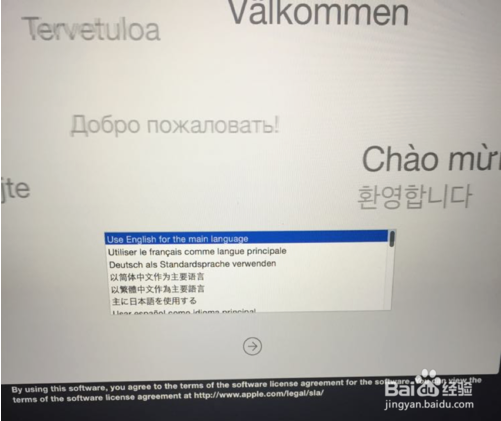
\includegraphics[width=0.8\textwidth]{figures/chushi.jpg}
  \label{chushi}
   \caption{初始进入界面}
   \end{figure}
\item 选择要安装的语言,点击继续
\item 连Wi-Fi,如图 \ref{wifi}
  \begin{figure}[!htb] %插图
  \centering
  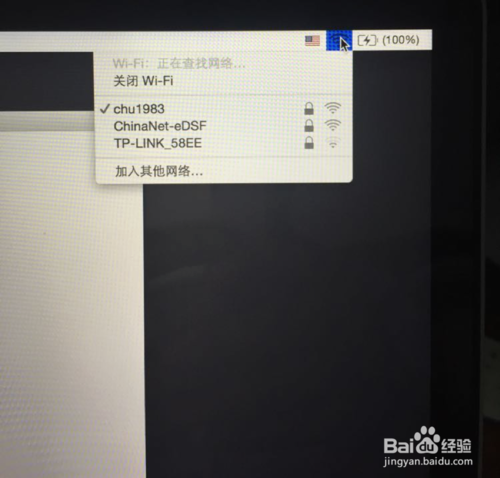
\includegraphics[width=0.8\textwidth]{figures/wifi.jpg}
  \label{wifi}
  \caption{连接网络}
  \end{figure}
\item 如图 \ref{cipangongju},点击【磁盘工具】
 \begin{figure}[!htb] %插图
 \centering
 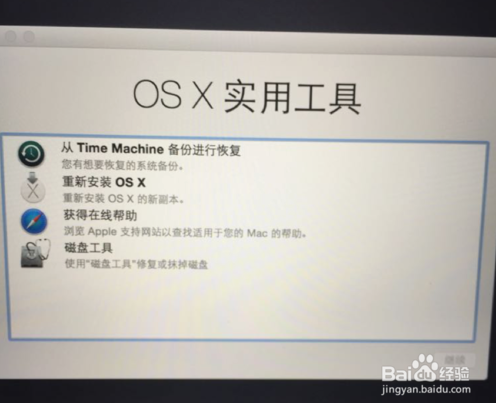
\includegraphics[width=0.8\textwidth]{figures/cipangongju.png}
 \label{cipangongju}
 \caption{OS X使用工具}
 \end{figure}
\item 点击第二个磁盘(Macintosh HD ),如下图\ref{hd} 鼠标的位置所示;【注意】如果您安装了Windows双系统,那么下图会出现第三个磁盘  (BOOTCAMP盘)这个不用抹掉,没有的话(下图中就没有)和不懂我在说什么的同志看下一步,没事;
 \begin{figure}[!htb] %插图
 \centering
 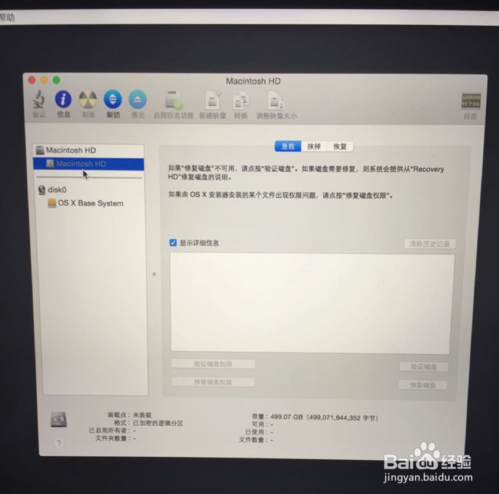
\includegraphics[width=0.8\textwidth]{figures/hd.png}
 \label{hd}
 \caption{磁盘工具界面}
 \end{figure}

\item 点击第二个磁盘(Macintosh HD )后,如下图\ref{modiao},选择中上方的“抹掉”选项卡 ,然后点击右下角的“抹掉…”。【注意】此步骤为格盘,也就是清空电脑的磁盘,把它变为全新空白的,电脑里所有软件和文件都将清空;
 \begin{figure}[!htb] %插图
 \centering
 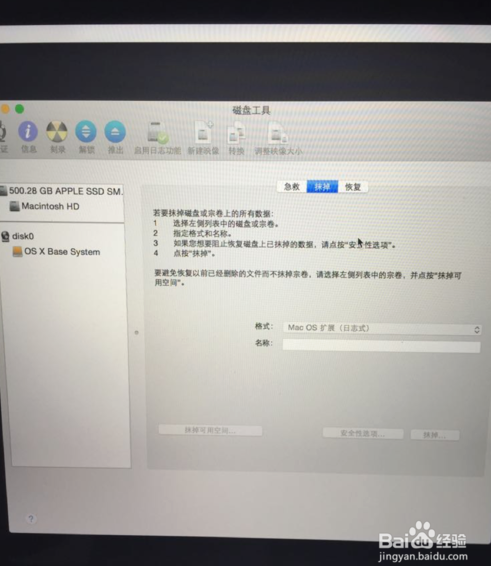
\includegraphics[width=0.8\textwidth]{figures/modiao.png}
 \label{modiao}
 \caption{格式化磁盘}
 \end{figure}

\item 如图\ref{jixu}关闭上面的窗口,选择【重新安装OS X】
 \begin{figure}[!htb] %插图
 \centering
 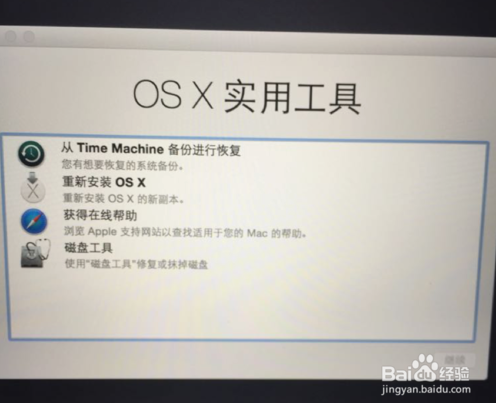
\includegraphics[width=0.8\textwidth]{figures/cipangongju.png}
 \label{jixu}
 \caption{重新安装OS X}
 \end{figure}

\item 如图\ref{jixuanzhuang},点击“继续”,后面的不用说了,选择“同意”之类的条款。
 \begin{figure}[!htb] %插图
 \centering
 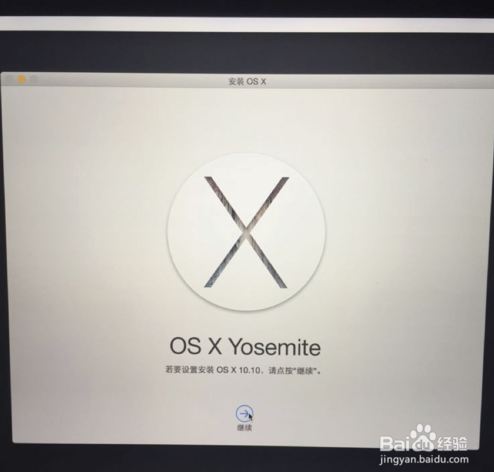
\includegraphics[width=0.8\textwidth]{figures/jixu.png}
 \label{jixuanzhuang}
 \caption{安装界面}
 \end{figure}

\item 直到到下面这个界面,图\ref{anzhuang}就可以放着去休息了。
 \begin{figure}[!htb] %插图
 \centering
 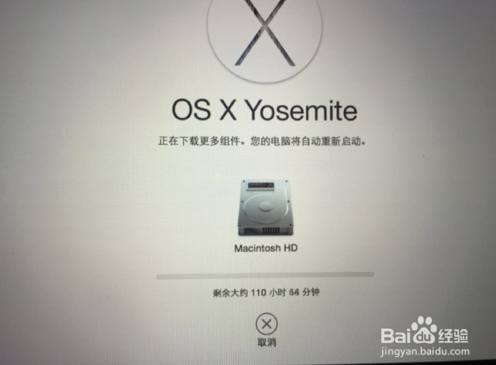
\includegraphics[width=0.8\textwidth]{figures/anzhuang.png}
 \label{anzhuang}
 \caption{安装界面}
 \end{figure}

\end{enumerate}

注意事项:

\begin{enumerate}

\item[a.] 不要关闭家里的无线(Wi-Fi)网络;

\item[b.] 整个过程要下载5个多GB的安装包,然后会全自动重装;

\item[c.] 上面写的还剩余多少小时不准确,几百个小时也别着急,因为连的是美国苹果官网,所以网速时快时慢;

\item[d.] 我们测试的重装速度情况是,中国大陆:最长6个小时自动重装完毕;中国香港:2个小时;英国:3个小时(欢迎大家补充);

\item[e.] 进度条满了之后,会全自动安装,不需要点击任何按钮,自动重装并进入新系统的。

\end{enumerate}

原贴地址:\url{http://jingyan.baidu.com/article/d71306352bb04713fdf4752a.html}

%========================================================================================================
\section{用安装盘进行系统安装}
\subsection{制作安装盘}

【准备工作】
\begin{enumerate}
\item U盘 16G以上(想要快请用 USB3.0)。\par     
注意:U盘的卷标名不要用中文!任何英文都可以。
\item MAC APP SOTRE 下载最新的OS X Yosemite 10.10~x(未来的新版也适用)。
\item 备份你的所有MACBOOK数据 。 
\end{enumerate}

【现在开始】
\begin{enumerate}
\item 插入U盘,打开“终端”。
如图\ref{tu1}所示。
\begin{figure}[!htb] %插图
\centering
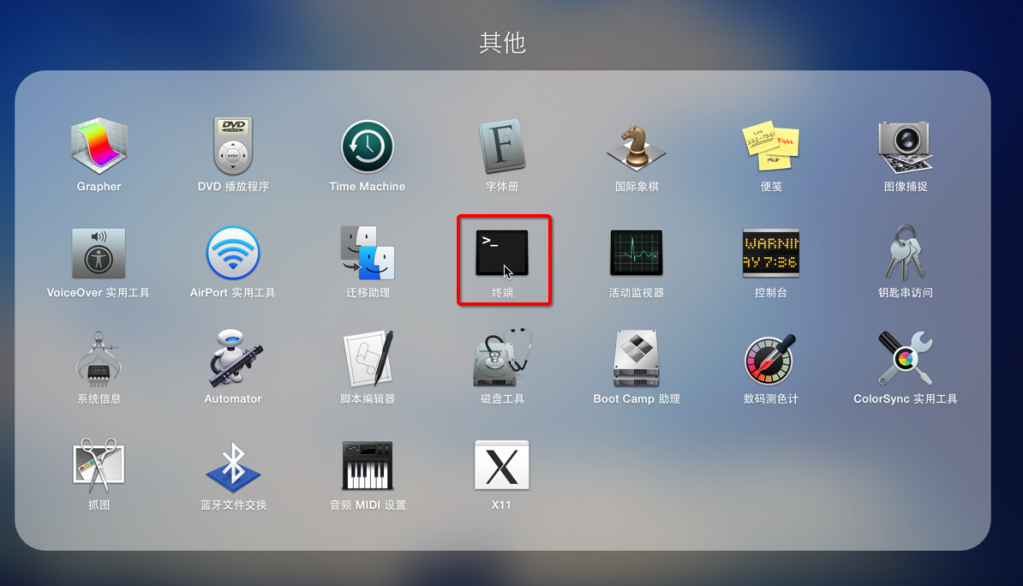
\includegraphics[width=0.5\textwidth]{figures/tu1.png}
\caption{运行结果}
\label{tu1}
\end{figure}
\item 在“终端”输入:sudo+空格。\par
tip: sudo 是提权的意思,将获得此台MACBOOK至高无上的权利。提示符也由 \# 变成 \$
如图\ref{tu2}所示。
\begin{figure}[!htb] %插图
\centering
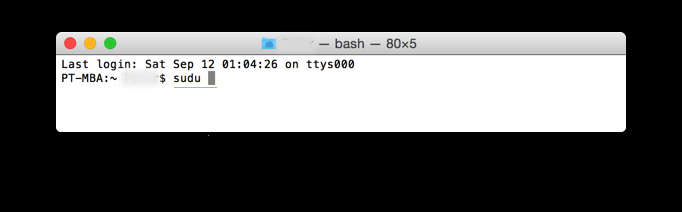
\includegraphics[width=0.7\textwidth]{figures/tu2.png}
\caption{运行结果}
\label{tu2}
\end{figure}
\item 找到OS X Yosemite.app安装包,右键选择“显示包内容”,在Contents/Resources/文件夹下找到:createinstallmedia 如图\ref{tu3}所示。
\begin{figure}[!htb] %插图
\centering
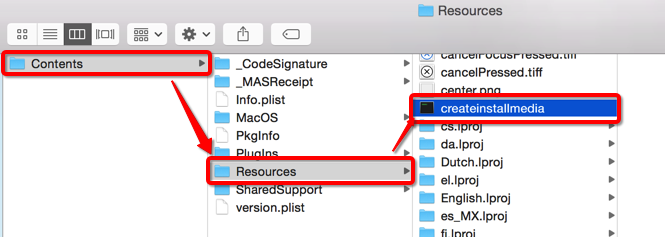
\includegraphics[width=0.7\textwidth]{figures/tu3.png}
\caption{运行结果}
\label{tu3}
\end{figure}
\item 将createinstallmedia文件拖入“终端”,如图\ref{tu4}所示。
\begin{figure}[!htb] %插图
\centering
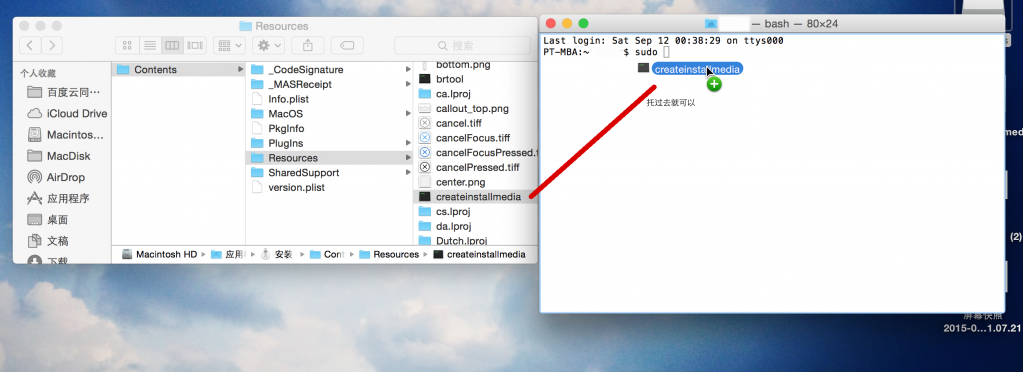
\includegraphics[width=1.1\textwidth]{figures/tu4.png}
\caption{运行结果}
\label{tu4}
\end{figure}
\item 输入 \verb|--|volume+空格 ,之后拖入U盘图标至“终端”,如图\ref{tu5}所示。
\begin{figure}[!htb] %插图
\centering
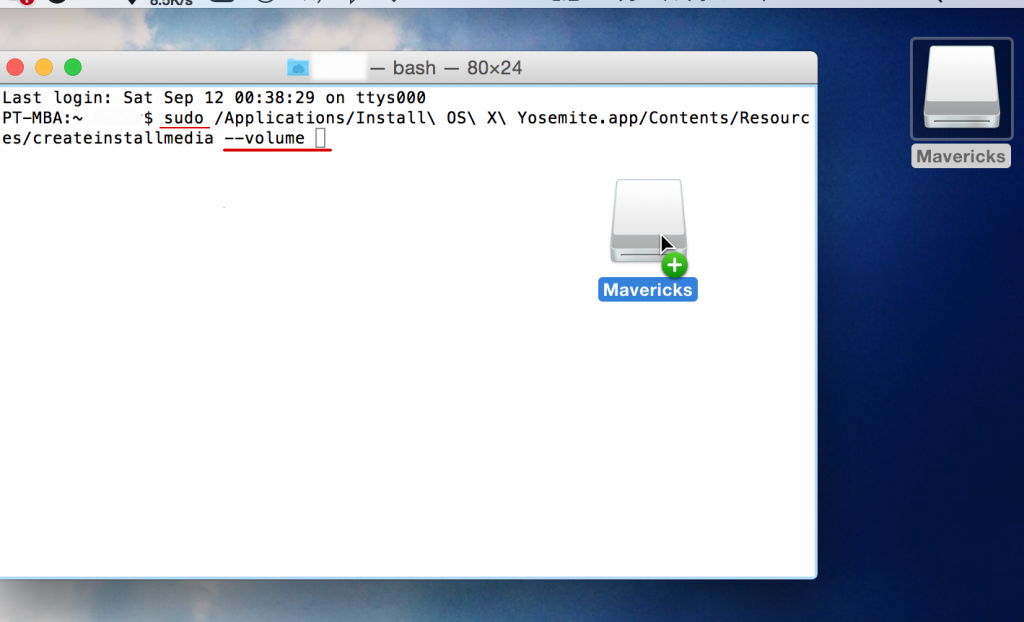
\includegraphics[width=0.7\textwidth]{figures/tu5.png}
\caption{运行结果}
\label{tu5}
\end{figure}
\item 输入 \verb|--|applicationpath+空格,之后将包拖入“终端”,如图\ref{tu6}所示。\par
OS X Yosemite.app 安装文件需要去MAC APP STORE去下载,一般在应用文件夹下面,如果是自已网上下载的就自行找到存储文件位置并拖入,如图\ref{tu6}所示。
\begin{figure}[!htb] %插图
\centering
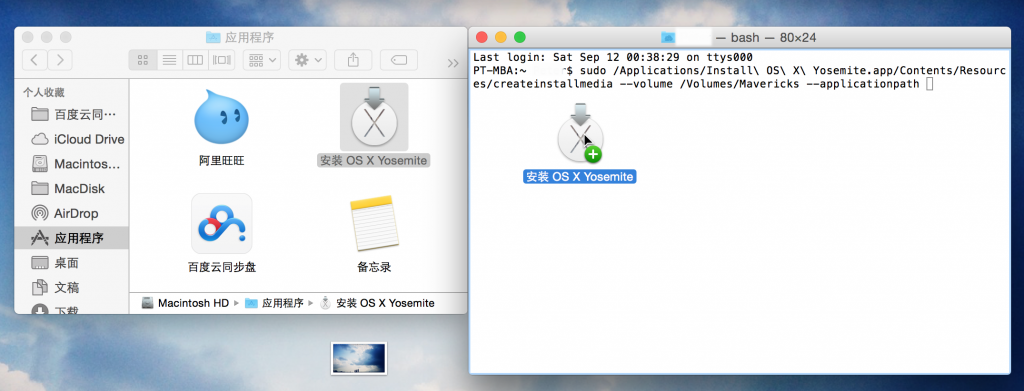
\includegraphics[width=1.1\textwidth]{figures/tu6.png}
\caption{运行结果}
\label{tu6}
\end{figure}
\item 最后输入 \verb|--|nointeraction,按“return”(回车),请看划线部份,系统会显示如图\ref{tu7}所示,并提示你输入电脑登录密码,如果没有密码直接按回车,如果看到DONE绿色框那里,就证明完成。\par
PS:copying installer files to disk.... 需要一点时间出现这样的提示,等待运行完成,显示 Done,制作安装盘完成。
\begin{figure}[!htb] %插图
\centering
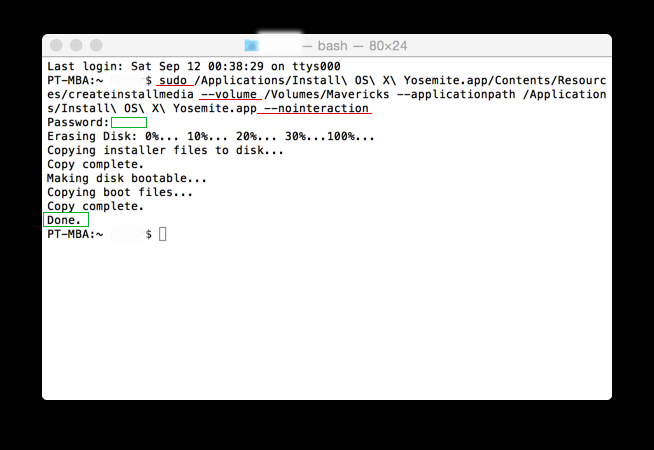
\includegraphics[width=0.8\textwidth]{figures/tu7.png}
\caption{运行结果}
\label{tu7}
\end{figure}\\
\end{enumerate}
【Q \& A 时间】
\begin{enumerate}
\item Q:有双系统的 MAC + WIN 会不会把WINDOWS格式掉?\par
   A:会,因为是全新安装
\item Q:制作MAC OS安装盘需要多久?\par
   A:  20分钟(USB2.0)
\item Q:换硬盘这个方法可以么?\par
   A:可以,重装系统空盘都行
\item Q:哪里有使用命令制作版本?\par
   A:苹果官方网站的链接:\url{https://support.apple.com/zh-cn/HT201372}
\end{enumerate}
\subsection{MAC 系统安装}
\begin{enumerate}
\item 点击左上角苹果图点,选重新启动,此时按住键盘上的OPTION键不放,等到启动界面中出现盘符选项的时候,用方向键选择刚制作好的U盘;经过几秒的运算,出现OS X实用工具界面,点击最下方的“磁盘工具”,打开磁盘工具,这时候我们要把老的系统格式化,这样装完的系统是全新的,会更干净流畅一点。格式化的方法和第一章介绍的方法一样。
\begin{figure}[!htb] %插图
\centering
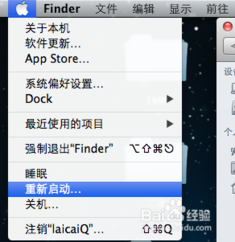
\includegraphics[width=0.4\textwidth]{figures/tu21.png}
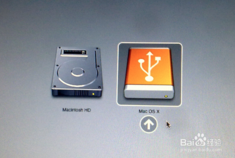
\includegraphics[width=0.4\textwidth]{figures/tu22.png}
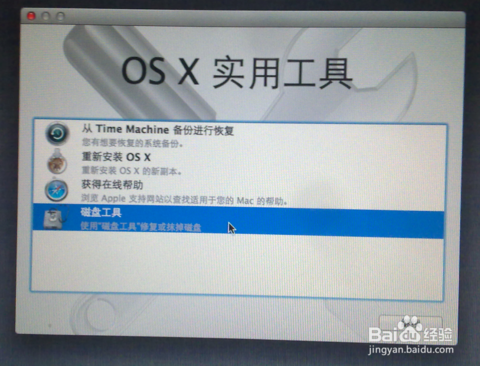
\includegraphics[width=0.4\textwidth]{figures/tu23.png}
\caption{\small 运行结果}
\label{tu21}
\end{figure} 
\item 关闭磁盘工具,回到os x 实用工具界面, 点击“重新安装os x" ,即开始安装,
如图\ref{tu28}所示。
\begin{figure}[!htb] %插图
\centering
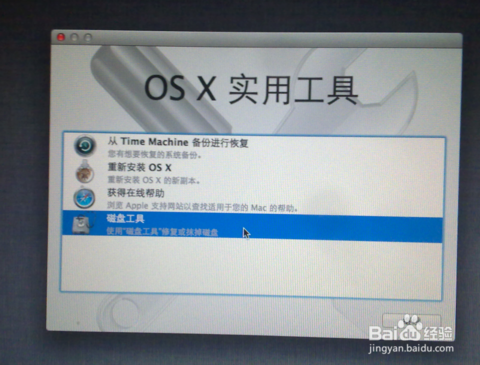
\includegraphics[width=0.4\textwidth]{figures/tu28.png}
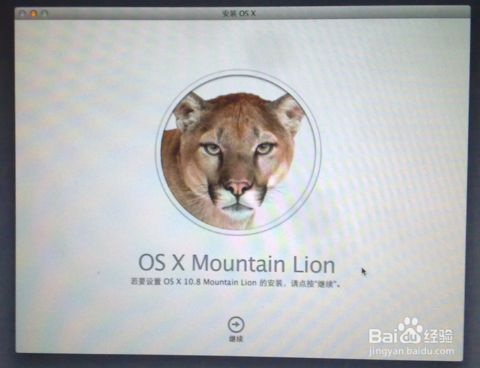
\includegraphics[width=0.4\textwidth]{figures/tu29.png}
\caption{\small 运行结果}
\label{tu28}
\end{figure}
\item 接下来,点击“同意”协议,选择安装的盘符到硬盘的盘符,接着,显示准备开始安装,大约二分钟之后,自动重启。
如图\ref{tu210}所示。
\begin{figure}[!htb] %插图
\centering
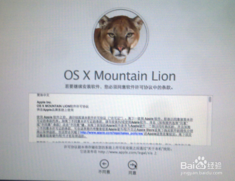
\includegraphics[width=0.3\textwidth]{figures/tu210.png}
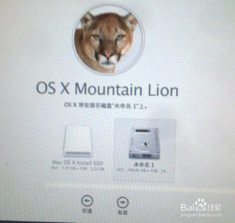
\includegraphics[width=0.3\textwidth]{figures/tu211.png}
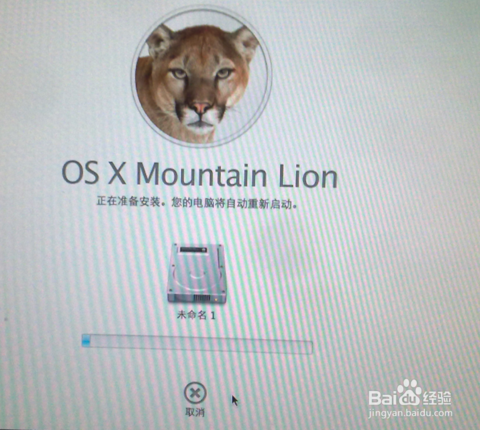
\includegraphics[width=0.3\textwidth]{figures/tu212.png}
\caption{\small 运行结果}
\label{tu210}
\end{figure} 
\item 重启之后,便开始正式安装,大约需要二十分钟的过程,装完后提示“安装完成”,然后重启,开始新系统的设置。
如图\ref{tu213}所示。
\begin{figure}[!htb] %插图
\centering
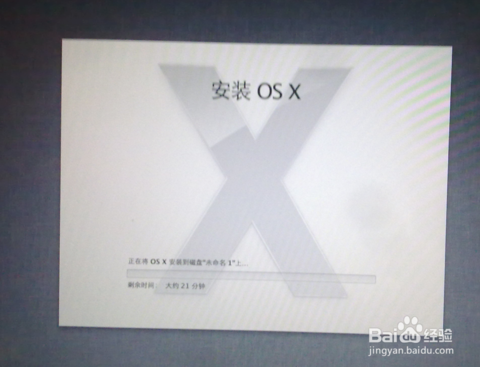
\includegraphics[width=0.3\textwidth]{figures/tu213.png}
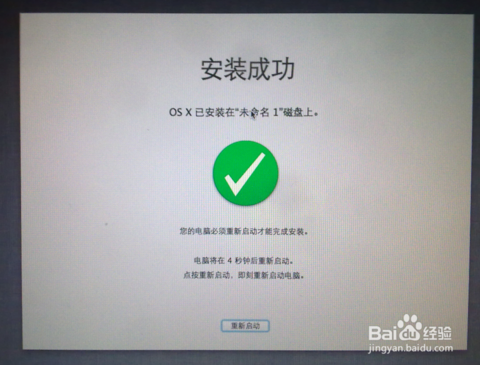
\includegraphics[width=0.3\textwidth]{figures/tu214.png}
\caption{\small 运行结果}
\label{tu213}
\end{figure} 
\item 重启之后,进入欢迎界面,逐步设置“地区”、“无线网”、“定位”以及“时区”等信息。
如图\ref{tu215}所示。
\begin{figure}[!htb] %插图
\centering
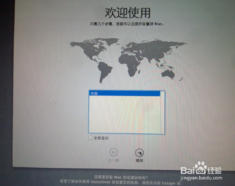
\includegraphics[width=0.3\textwidth]{figures/tu215.png}
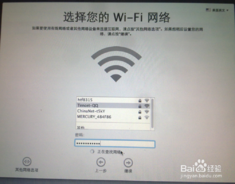
\includegraphics[width=0.3\textwidth]{figures/tu216.png}
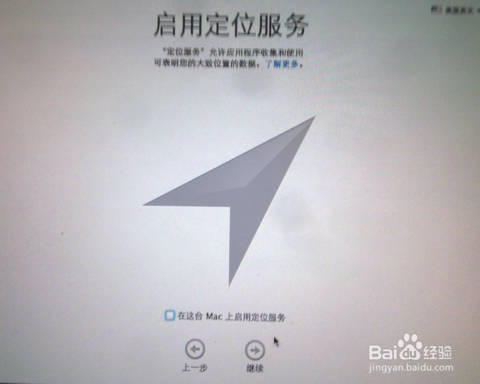
\includegraphics[width=0.3\textwidth]{figures/tu217.png}
\caption{\small 运行结果}
\label{tu215}
\end{figure} 
\item 完成一系列的设置,终于进入漂亮的系统桌面,桌面上除了dock什么内容也没有,我们从“偏好设置”中,把“硬盘”调出来,还可以根据个人喜好进行一系列的用户设置,新系统安装完成了,尽情享受吧!
如图\ref{tu218}所示。
\begin{figure}[!htb] %插图
\centering
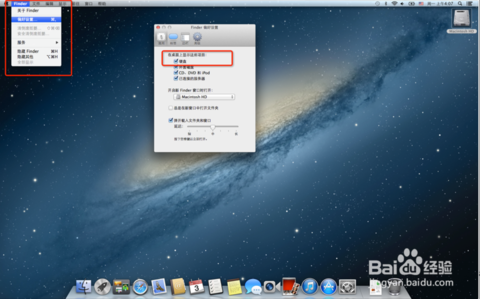
\includegraphics[width=0.5\textwidth]{figures/tu218.png}
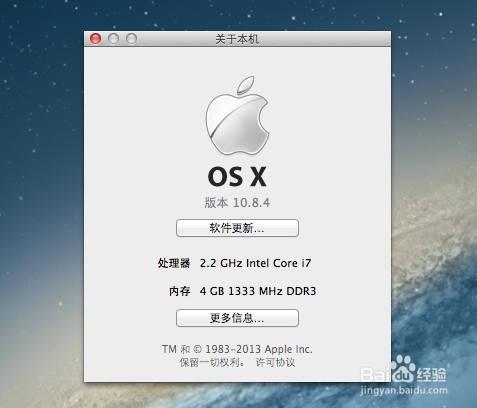
\includegraphics[width=0.4\textwidth]{figures/tu219.png}
\caption{\small 运行结果}
\label{tu218}
\end{figure} 
\end{enumerate}

\end{document}
